%%%%%%%%%%%%%%%%%%%%%%%%%%%%%%%%
% Chap 2. Related works of action recognition
%%%%%%%%%%%%%%%%%%%%%%%%%%%%%%%%

\chapter{The chapter 2}\label{chapter2}

Write your chapter 2. Write your chapter 2. Write your chapter 2. Write your chapter 2. Write your chapter 2. Write your chapter 2. Write your chapter 2. Write your chapter 2. Write your chapter 2. Write your chapter 2. Write your chapter 2. Write your chapter 2. Write your chapter 2. Write your chapter 2. Write your chapter 2. Write your chapter 2. Write your chapter 2. Write your chapter 2. 

\begin{figure}
\centering
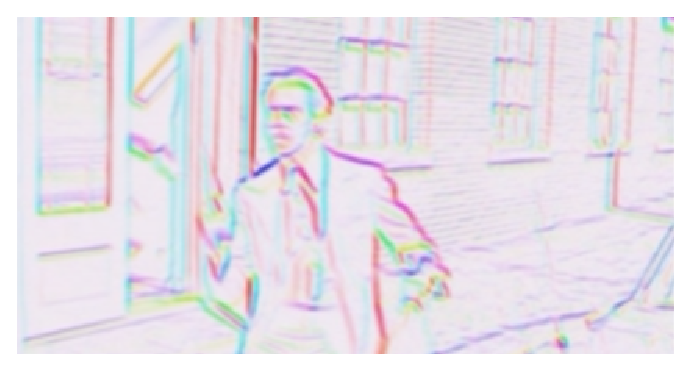
\includegraphics[scale=0.5]{imgs/HOG.eps}
\caption{An eps image}
\label{fig:hog}
\end{figure}

\section{A section} \label{chap2:sec1}
\subsection{A subsection} \label{sec1:1-1}

write what you did.


\begin{algorithm}[H]
  \KwData{this text}
  \KwResult{how to write algorithm with \LaTeX2e }
  initialization\;
  \While{not at end of this document}{
    read current\;
    \eIf{understand}{
      go to next section\;
      current section becomes this one\;
    }{
      go back to the beginning of current section\;
    }
  }
  \caption{How to write algorithms 1}
\end{algorithm}


Hi, hello, nice to meet you. Hi, hello, nice to meet you. Hi, hello, nice to meet you. Hi, hello, nice to meet you. Hi, hello, nice to meet you. Hi, hello, nice to meet you. Hi, hello, nice to meet you. Hi, hello, nice to meet you. Hi, hello, nice to meet you. Hi, hello, nice to meet you. Hi, hello, nice to meet you. Hi, hello, nice to meet you. 

